\setcounter{section}{2}
\setcounter{subsection}{0}

\sectionVKR{Проектирование приложения}

\subsection{Пользовательские сценарии}

В этом разделе представлены сценарии использования разрабатываемого сервиса, демонстрирующие взаимодействие пользователя с системой. Диаграмма прецедентов изображена на рисунке \ref{pic:uc}.

\subsubsection{Сценарии исследователя}

Создание лабораторного эксперимента позволяет учёному сформировать новый эксперимент с подробным описанием и таблицей измерений. После выбора опции “Создать лабораторный эксперимент” пользователь вводит описание эксперимента и может добавить таблицу с измерениями. В таблице столбцы могут быть привязаны к соответствующим онтологиям, например, для указания единиц измерения или терминов. После завершения работы с таблицей и описанием, исследователь сохраняет эксперимент в системе для дальнейшего анализа.

Создание шаблона вычислительного эксперимента выглядит так: исследователь выбирает опцию “Создать шаблон вычислительного эксперимента” и вводит описание название эксперимента. Затем добавляются схемы для входных данных, выходных данных, параметров эксперимента и дополнительного контекста. Все эти данные привязываются к онтологиям для правильной обработки и отображения. После заполнения шаблона и конкретных данных, эксперимент сохраняется для дальнейшей работы.

Создание запуска вычислительного эксперимента доступно через опцию “Создать запуск вычислительного эксперимента”. Вычислительный эксперимент заполняется по созданному шаблону с уже реальными входными и выходными данными, а также с параметрами, которые необходимы для вычислительного процесса и опциональным дополнительным контекстом.

Работа с онтологиями представляет собой привязку различных элементов данных к онтологическим терминам. В процессе исследователь может выбрать столбцы таблицы или параметры эксперимента в шаблоне вычислительного эксперимента, которые должны быть связаны с конкретной онтологией. После выбора подходящего термина из онтологии, система автоматически привязывает его к выбранному элементу данных.

Получение описания терминов при наведении предоставляет исследователю дополнительную информацию о терминах, используемых в эксперименте. Когда пользователь наводит курсор на термин, привязанный к столбцу таблицы или элементу данных, система отображает всплывающее окно с кратким описанием этого термина. Описание содержит информацию о единице измерения, значении термина или других деталях, что помогает исследователю быстрее разобраться в значении терминов.

Регистрация и авторизация являются обязательными этапами перед выполнением всех остальных действий в системе. На первом этапе пользователь проходит процесс регистрации, заполняя необходимые данные: логин, электронную почту и пароль. При отсутствии пользователя с указанной электронной почтой регистрация завершается успешно. В процессе авторизации он вводит свои учетные данные (логин и пароль), и система проверяет их на корректность. Только после успешной авторизации пользователь получает доступ к функционалу системы, в зависимости от своей роли.

Экспорт данных позволяет исследователю передавать результаты эксперимента в различных форматах для дальнейшего использования или анализа. После завершения работы с экспериментом, пользователь выбирает опцию экспорта, где можно выбрать один из форматов — CSV, JSON или PDF. Система генерирует файл в выбранном формате, который затем можно скачать.

\subsubsection{Сценарии администратора}

Управление пользователями позволяет администратору системы добавлять и редактировать пользователей, а также назначать им соответствующие роли. Администратор может регулировать, кто может просматривать, редактировать или просматривать эксперименты, также назначить различные уровни доступа для разных пользователей.

\begin{figure}[H]
    \centering
    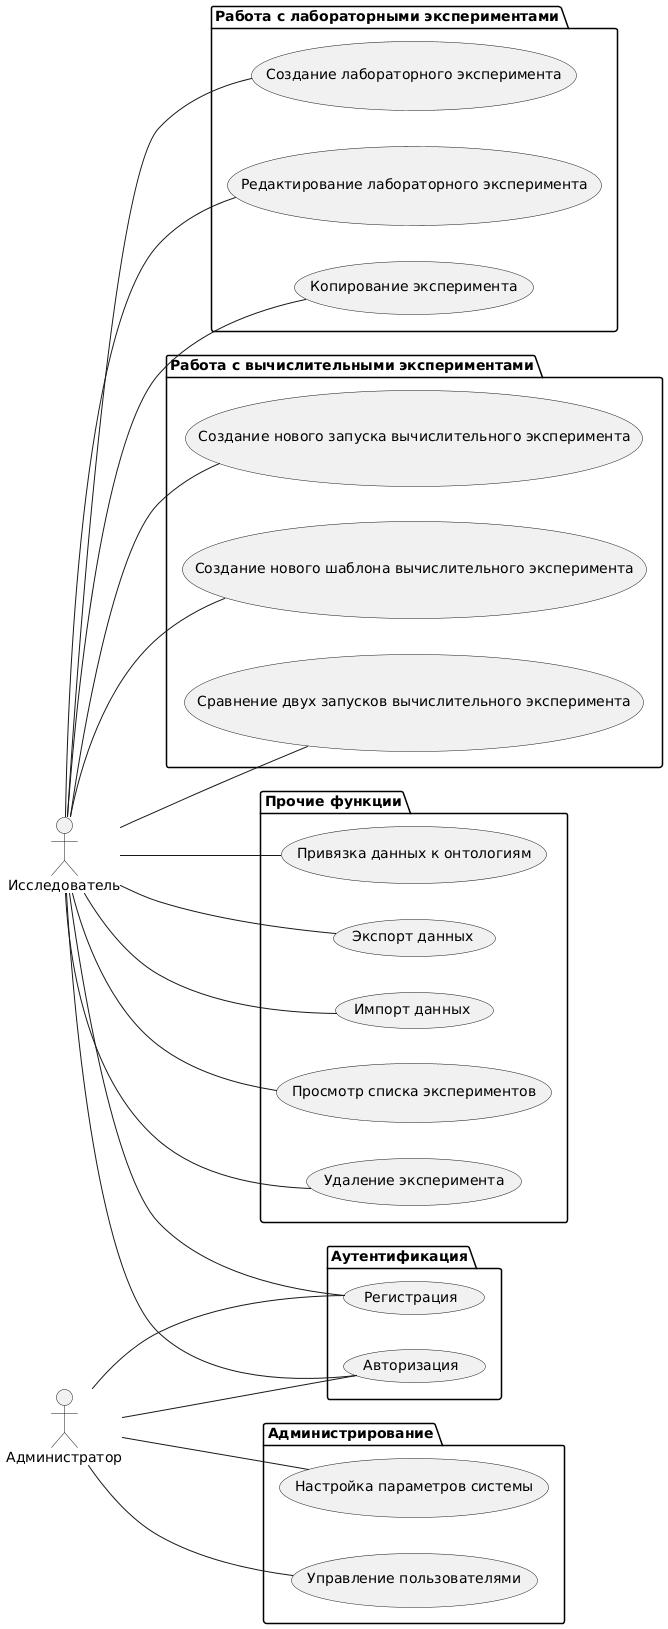
\includegraphics[width=0.5\linewidth]{img/use_cases.png}
    \caption{Диаграмма пользовательских сценариев}
    \label{pic:uc}
\end{figure}

\subsection{Архитектура приложения}

\subsubsection{Схема базы данных}

Таблица \texttt{users} хранит информацию о пользователях системы. Поле \texttt{id} является уникальным идентификатором пользователя. \texttt{username} содержит имя пользователя, а \texttt{username} — его уникальный никнейм. \texttt{hashed\_password} используется для хранения зашифрованного пароля. Поле \texttt{role} указывает на роль пользователя в системе.

Таблица \texttt{lab\_experiments} предназначена для хранения лабораторных экспериментов. \texttt{id} — уникальный идентификатор эксперимента. \texttt{title} содержит название эксперимента, а \texttt{description} — его описание. Поле \texttt{user\_id} указывает на пользователя, создавшего эксперимент. \texttt{created\_at} фиксирует дату и время создания записи.

Таблица \texttt{measurement} используется для хранения результатов измерений в лабораторных экспериментах. \texttt{id} — уникальный идентификатор записи. \texttt{experiment\_id} указывает, к какому лабораторному эксперименту относится измерение. \texttt{pivot\_key} определяет категорию данных. \texttt{parameter} хранит название измеряемого параметра, \texttt{value} содержит его числовое или текстовое значение. Поле \texttt{unit} связано с таблицей \texttt{ontology} и определяет единицу измерения.

Таблица \texttt{ontology} предназначена для хранения онтологических данных. Поле \texttt{id} является уникальным идентификатором онтологического термина. \texttt{name} содержит название термина, \texttt{dimension} — его размерность (например, масса, длина), а \texttt{uri} — ссылку на онтологический ресурс.

Таблица \texttt{computational\_experiments} хранит вычислительные эксперименты. \texttt{id} — уникальный идентификатор. \texttt{title} содержит название, а \texttt{description} — описание эксперимента. \texttt{user\_id} указывает на владельца эксперимента. Поле \texttt{created\_at} фиксирует дату создания, а \texttt{template\_id} связывает эксперимент с шаблоном из таблицы \texttt{computational\_templates}.

Таблица \texttt{computational\_experiment\_data} содержит конкретные данные вычислительных экспериментов. Поле \texttt{experiment\_id} связывает данные с конкретным экспериментом. \texttt{input\_data} хранит входные данные в формате JSON. \texttt{output\_data} содержит выходные данные, \texttt{parameters} включают параметры модели, а \texttt{context} — дополнительные сведения, не привязанные к онтологиям.

Таблица \texttt{computational\_templates} определяет шаблоны вычислительных экспериментов. Поле \texttt{id} является уникальным идентификатором, а \texttt{title} содержит название шаблона.

Таблица \texttt{computational\_experiment\_schemas} описывает схемы данных для вычислительных экспериментов. Поле \texttt{template\_id} связывает схему с соответствующим шаблоном. \texttt{input\_schema} определяет структуру входных данных в формате JSON, \texttt{output\_schema} — выходных, \texttt{parameter\_schema} описывает параметры эксперимента, а \texttt{context\_schema} задает структуру дополнительных данных.

Общая схема базы данных представлена на рисунке \ref{pic:db}.

\begin{figure}[H]
	\centering
	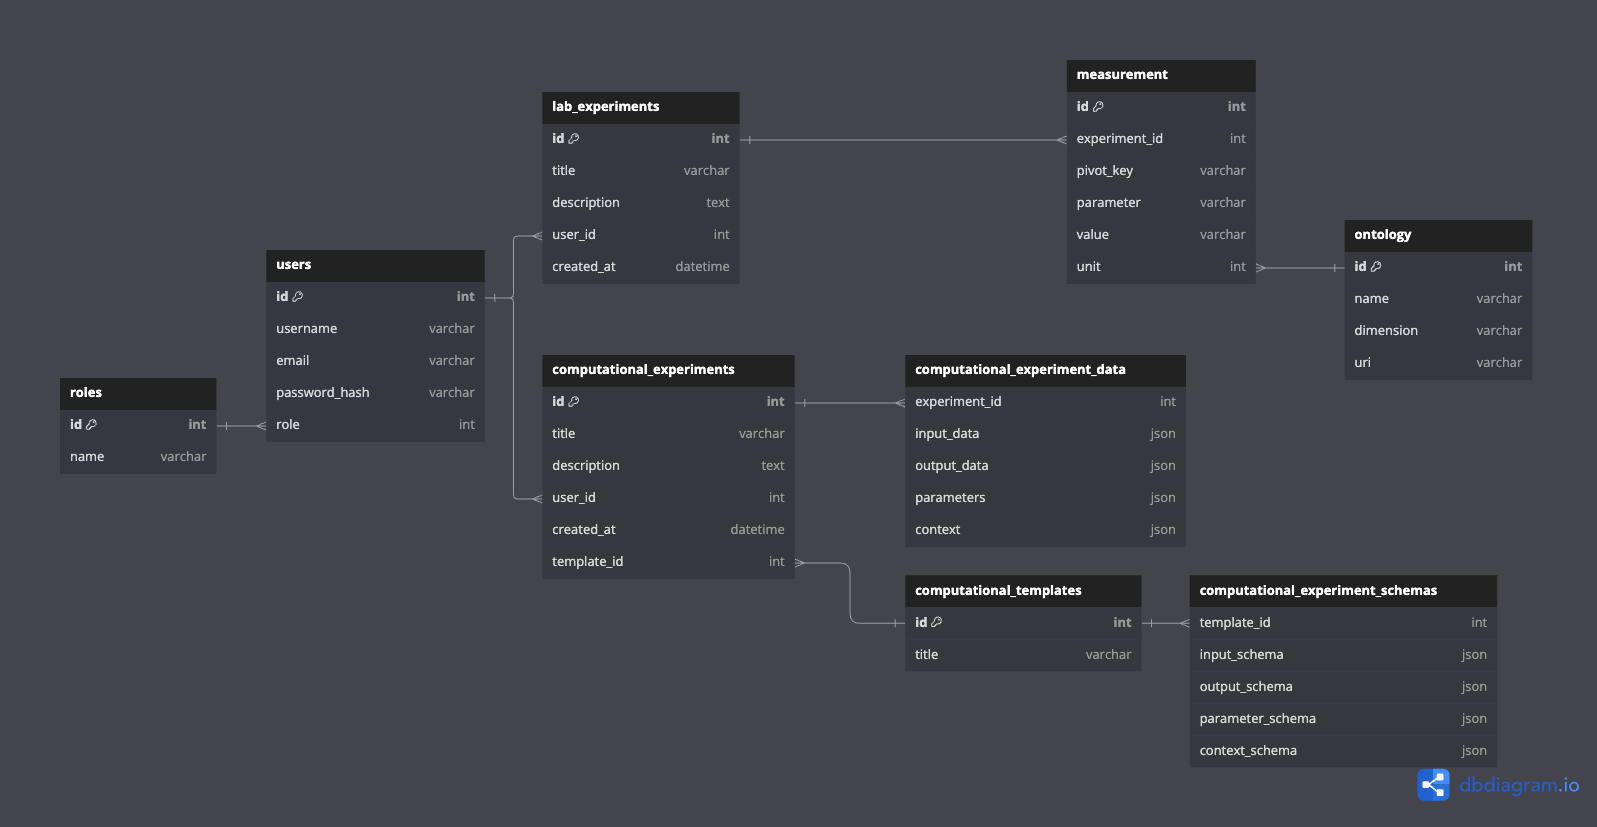
\includegraphics[width=\linewidth]{chapters/img/database_scheme.png}
	\caption{Схема базы данных}
	\label{pic:db}
\end{figure}


\subsubsection{Архитектура серверного приложения}

Выбранная архитектура приложения изображена на рисунке \ref{pic:server_arch} и основана на слоистом подходе, который обеспечивает разделение ответственности между компонентами, улучшает модульность и делает систему более поддерживаемой и масштабируемой. В серверной части реализована организация слоев: API Router обрабатывает входящие HTTP-запросы и передает их в слой бизнес-логики, где осуществляется основная обработка данных. Для работы с базами данных используется слой доступа к данным, который взаимодействует с PostgreSQL и Neo4j. Дополнительно выделены сервис аутентификации и уровень валидации, что обеспечивает безопасность и корректность данных.

\begin{figure}[H]
	\centering
	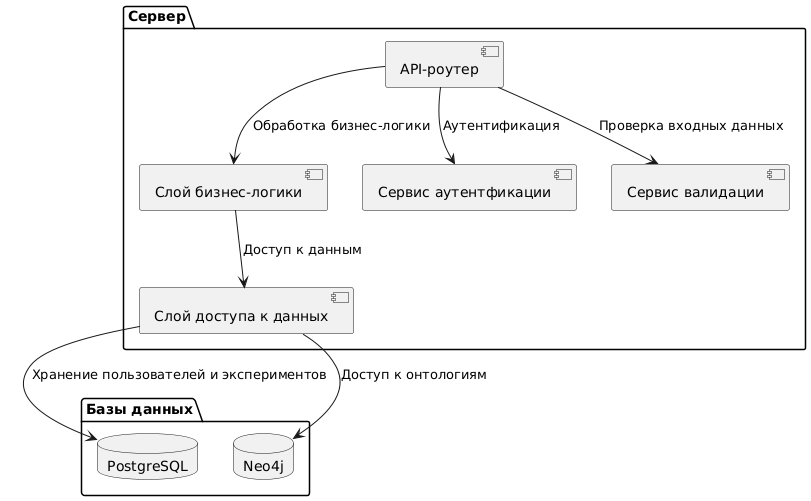
\includegraphics[width=0.7\linewidth]{chapters/img/server_arch.png}
	\caption{Архитектура серверного приложения}
	\label{pic:server_arch}
\end{figure}

\subsubsection{Архитектура клиентского приложения}

Клиентская часть построена на Vue.js и также следует принципам разделения ответственности. Компоненты пользовательского интерфейса взаимодействуют с хранилищем состояния (Pinia\cite{Library:Pinia}), которое управляет данными и их синхронизацией. Взаимодействие с сервером осуществляется через API Service, что позволяет отделить сетевые запросы от логики компонентов, а Vue Router\cite{Library:VueRouter} управляет навигацией. Такой подход обеспечивает гибкость и удобство в разработке. Архитектура клиентской части изображена на рисунке \ref{pic:client_arch}.

\begin{figure}[H]
	\centering
	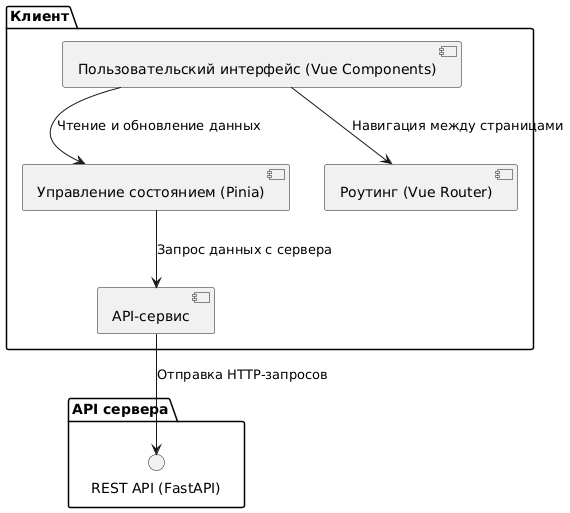
\includegraphics[width=\linewidth]{chapters/img/client_arch.png}
	\caption{Архитектура клиентского приложения}
	\label{pic:client_arch}
\end{figure}

\subsection{Выбор методов и средств реализации}

При выборе технологий для разработки веб-приложения учитывались следующие ключевые факторы:
\begin{enumerate}
    \item Производительность и масштабируемость.
    \item Простота интеграции с онтологиями.
    \item Поддержка современных стандартов веб-разработки.
    \item Лёгкость развертывания и сопровождения.
\end{enumerate}

На основании этих критериев были выбраны следующие технологии:

\subsubsection{Выбор фреймворка для серверной части}

В качестве веб-фреймворка для бэкенда было выбрано FastAPI по следующим причинам:
\begin{enumerate}
    \item Высокая производительность — благодаря использованию Starlette~\cite{Framework:Starlette} и Pydantic~\cite{Library:Pydantic}, FastAPI демонстрирует скорость работы, сопоставимую с Node.js~\cite{Lang:NodeJS} и Go~\cite{Lang:Go}, что особенно важно при работе с API для экспериментов.
    \item Асинхронная обработка запросов — поддержка async/await позволяет обрабатывать несколько запросов одновременно без блокировки потока выполнения, что критично при обработке вычислительных экспериментов.
    \item Встроенная валидация данных — благодаря Pydantic, валидация данных выполняется на уровне схем API, уменьшая вероятность ошибок на клиенте и сервере.
    \item Гибкость в интеграции — поддержка OpenAPI и облегчает документирование и подключение к клиентской части.
\end{enumerate}

Альтернативными вариантами были Django Rest Framework (DRF)~\cite{Framework:DRF} и Flask~\cite{Framework:Flask}, однако:
\begin{enumerate}
    \item DRF имеет более сложную архитектуру и высокие накладные расходы по сравнению с FastAPI.
    \item Flask не поддерживает асинхронную обработку из коробки, что снижает его эффективность для API с высокой нагрузкой.
\end{enumerate}

\subsubsection{Выбор фреймворка для клиентской части}

Для реализации фронтенда было выбрано Vue.js (Composition API) вместо React~\cite{Framework:React} и Angular~\cite{Framework:Angular}. Основные причины выбора:
\begin{enumerate}
    \item Лёгкость освоения и высокая продуктивность — Vue.js имеет интуитивно понятный синтаксис и гибкость в использовании как декларативного программирования, так и компонентов.
    \item Композиционный API — использование Composition API в Vue 3 улучшает переиспользуемость кода и упрощает управление состоянием.
    \item Высокая производительность — виртуальный DOM оптимизирован, механизм реактивности позволяет минимизировать ререндеринг.
    \item Гибкость в архитектуре — Vue.js легко интегрируется с серверными приложениями через REST API.
\end{enumerate}

Альтернативами рассматривались:
\begin{enumerate}
    \item React — мощный, но требует дополнительной конфигурации и использования сторонних библиотек для маршрутизации и управления состоянием.
    \item Angular — мощный, но имеет высокие накладные расходы на разработку.
\end{enumerate}

\subsubsection{Выбор библиотеки для пользовательского интерфейса}

Библиотека компонентов PrimeVue~\cite{Framework:PrimeVue} выбрана для реализации интерфейса по следующим причинам:
\begin{enumerate}
    \item Готовые UI-компоненты — ускоряет разработку благодаря наличию таблиц, форм, модальных окон и других элементов.
    \item Поддержка тем — пакет предоставляет несколько готовых тем, позволяющих легко менять визуальное оформление.
    \item Гибкость — компоненты адаптируются под мобильные и десктопные устройства.
\end{enumerate}

Альтернативой был Vuetify, но он менее гибок по сравнению с PrimeVue.

\subsubsection{Выбор реляционной СУБД}

В качестве основной базы данных была выбрана PostgreSQL, поскольку:
\begin{enumerate}
    \item Поддерживает сложные реляционные структуры — идеально подходит для хранения экспериментов, пользователей и привязок к онтологиям.
    \item Расширенные возможности JSONB — позволяет эффективно хранить и обрабатывать JSON-документы без использования NoSQL-решений.
    \item Высокая производительность — оптимизированные индексы и транзакции позволяют обрабатывать большие объёмы данных.
\end{enumerate}

Наиболее конкурентоспособная альтернатива – MySQL~\cite{DB:MySQL}, но данная СУБД хуже работает с JSONB и менее стабилен при высоких нагрузках.

\subsubsection{Выбор графовой СУБД}

Так как приложение активно работает с онтологиями, было принято решение использовать Neo4j для хранения и обработки онтологических связей:
\begin{enumerate}
    \item Графовая структура — идеально подходит для представления онтологий, где между сущностями существует множество взаимосвязей.
    \item Cypher Query Language~\cite{QueryLang:CypherQL} — позволяет легко выполнять сложные запросы, например, нахождение зависимостей между измерениями.
    \item Гибкость — позволяет расширять базу знаний без нарушения структуры данных.
    \item Плагин neosemantics~\cite{Library:NeoSemantics} – позволяет удобно работать с онтологиями, представленными в RDF/XML.
\end{enumerate}

\subsubsection{Выбор средств развёртывания}

Для контейнеризации приложения используется Docker Compose~\cite{Tool:DockerCompose}, по следующим причинам:
\begin{enumerate}
    \item Простота конфигурации — управление контейнерами через docker-compose.yml не требует сложных манифестов.
    \item Более удобен для разработки — локальная среда легко воспроизводится на разных машинах.
    \item Не требует дополнительного оркестратора — Kubernetes~\cite{Tool:Kubernetes} сложен в настройке и требует значительных ресурсов.
    \item Быстрое развертывание — приложение запускается одной командой, обеспечивая автоматический запуск всех сервисов.
\end{enumerate}

Kubernetes рассматривался как альтернатива, но его сложность оправдана только для высоконагруженных распределённых систем, что не является текущей целью проекта.

\anonsubsection{Выводы по главе}

В этой главе рассмотрены сценарии использования системы и её архитектура на разных уровнях. Подробно описана структура компонентов, их взаимодействие, а также ключевые аспекты разработки, включая выбор технологий и проектные решения.